\documentclass[../DoAn.tex]{subfiles}
\begin{document}
Chương 1 đã giới thiệu tổng quan, nhu cầu cần thiết và nhiệm vụ chính của bài toán tích hợp dữ liệu nói chung và bài toán so sánh giá các sản phẩm Apple nói riêng. Chương 2 này sẽ trình bày về khảo sát hiện trạng và yêu cầu của phần mềm ứng dụng sau đó tiến hành so sánh phân tích ưu nhược điểm của các hệ thống đã khảo sát. Bên cạnh đó chương này sẽ tóm tắt các các chức năng cơ bản của hệ thống so sánh giá.

\section{Khảo sát hiện trạng}
\label{section:2.1}
Giá cả là yếu tố được người tiêu dùng quan tâm khi có ý định mua sắm và sử dụng bất kỳ sản phẩm hay dịch vụ nào. Các website so sánh giá trưc tuyến ra đời nhằm hỗ trợ người tiêu dùng trong việc dễ dàng tham khảo các mức giá và thông tin chi tiết của sản phẩm để mua sắm hợp lý hơn. Website so sánh giá là một website dạng tiếp thị, quảng bá được xem như một công cụ tìm kiếm cho phép người dùng so sánh giá của sản phẩm mình quan tâm trên các gian hàng trực tuyến khác nhau. Mục đích của người dùng khi sử dụng các trang web so sánh giá  là có thể mua được sản phẩm ở một nơi bán uy tín với mức giá rẻ nhất về mặt chất lượng. Hầu hết các trang web so sánh đều không trực tiêp bán hàng. Chúng chỉ liệt kê các gian hàng, cửa hàng trực tuyến cùng bán một sản phẩm với mức giá khác nhau để người dùng tìm hiểu và lựa chọn.

Hiện nay, đối với bài toán tích hợp dữ liệu ứng dụng vào so sánh giá các loại sản phẩm có rất nhiều nổi bật có thể kể đến như websosanh.vn, sosanhgia.com, topgia.vn, gobear,… Các hệ thống so sánh giá này rất đa dạng về các loại sản phẩm, dữ liệu từ nhiều nguồn tích hợp lại với nhau cho phép người dùng so sánh giá giữa các bên cung cấp khác nhau cũng như giá cập nhật tại một thời điểm. Để thực hiện các chức năng đó, hệ thống được thiết kế theo kiến trúc tích hợp dữ liệu ảo (Virtual data integration) xử lý các truy vấn và tích hợp dữ liệu tại thời điểm truy vấn. Tuy nhiên nó vẫn có một số nhược điểm như việc tìm kiếm các sản phẩm cụ thể (thông tin về cấu hình đối với điện thoại, ipad, máy tính, …) cho kết quả độ chính xác không cao. Vì tích hợp dữ liệu tại thời điểm xử lý truy vấn nên tốc độ xử lý sẽ chậm hơn tùy thuộc vào số lượng nguồn xử lý ,… Bên cạnh đó một số web so sánh là thiếu khách quan vì các gian hàng, cửa hàng phải trả phí để sản phẩm của họ được hiển thị. Việc này cũng làm xuất hiện nhiều gian hàng ảo, cố tình sử dụng lỗ hổng để thu hút khách hàng. Trong khi đó có nhiều gian hàng chất lượng tốt giá rẻ hơn lại không được xuất hiện vì không tham gia trả phí.

Xác định được hiện trạng và nhu cầu của người dùng, trong đồ án này em quyết định xây dựng hệ thống tích hợp dữ liệu sản phẩm Apple theo hướng tiếp cận data warehouse khắc phục những nhược điểm trên giúp cho việc truy vấn dữ liệu nhanh chóng và có độ chính xác cũng như gần nhất với yêu cầu của người dùng. Hệ thống tập trung vào xây dựng một kho dữ liệu các sản phẩm Apple cho phép người dùng có thể tìm kiếm với nhiều lựa chọn hơn như tên, dung lượng bộ nhớ trong, dung lượng bộ nhớ ngoài, màu sắc, và trạng thái sản phẩm.

\section{Tổng quan chức năng}
\label{section:2.2}
Phần \ref{section:2.2} này có nhiệm vụ tóm tắt các chức năng của phần mềm. Trong phần này chỉ mô tả chức năng mức cao (tổng quan) mà không đặc tả chi tiết cho từng chức năng. Đặc tả chi tiết được trình bày trong phần \ref{section:2.3}.

\subsection{Biểu đồ use case tổng quát}
\label{subsection:2.2.1}
Phần mềm có một tác nhân người dùng. Người dùng ở đây có thể là bất kì ai muốn tìm kiếm so sánh giá các sản phẩm Apple mà không cần đăng kí đăng nhập vào hệ thống.

% 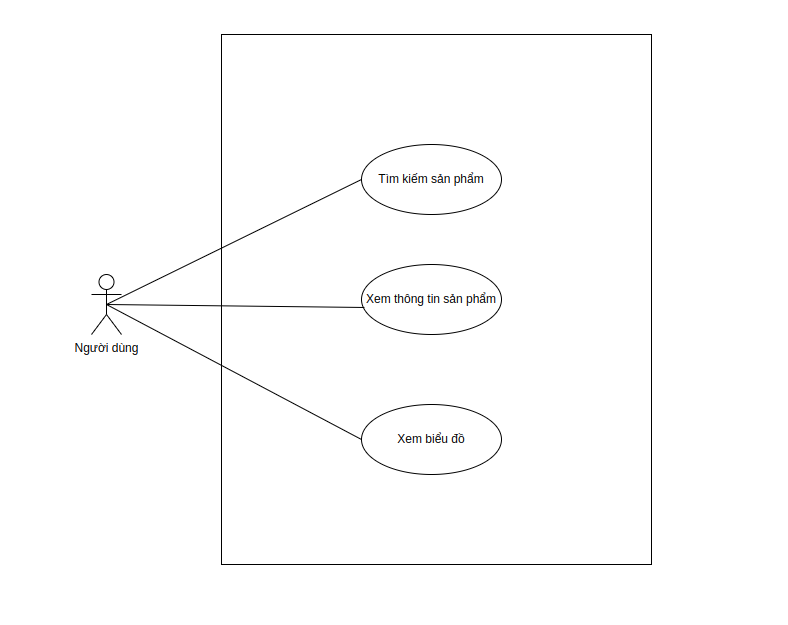
\includegraphics[scale=.6]{Hinhve/usecase.png}
\begin{figure}[H]
    \centering
    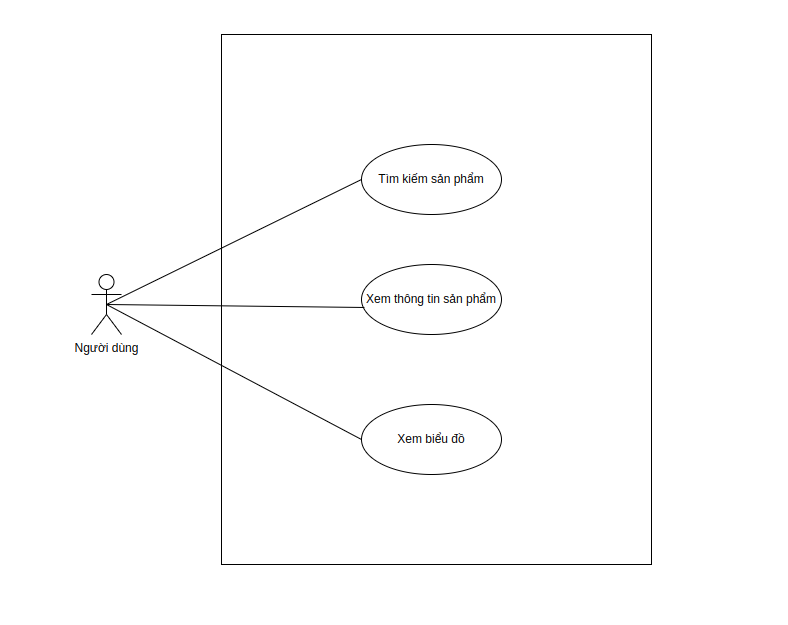
\includegraphics[scale=.6]{Hinhve/usecase.png}
    \caption{Usecase tìm kiếm sản phẩm}
    \label{fig:my_label2}
\end{figure}

Phầm mềm có 3 chức năng chính: Tìm kiếm sản phẩm bằng các lọc các trường tên, màu sắc,.. Người dùng cũng có thể xem thông tin chi tiết sản phẩm và biểu đồ phân tích thị trường.
\subsection{Biểu đồ use case phân rã Tìm kiếm sản phẩm}
\label{subsection:2.2.2}
Biểu đồ use case phân rã Tìm kiếm sản phẩm

% 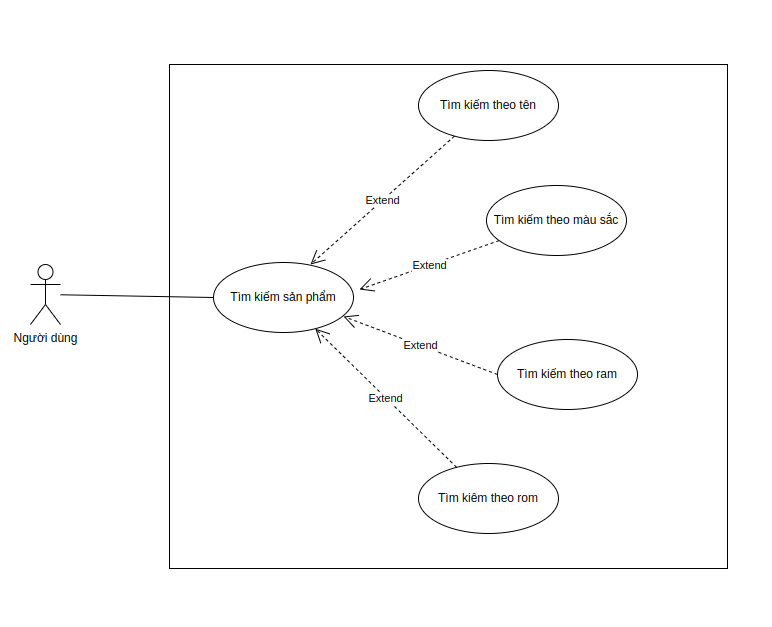
\includegraphics[scale=0.6]{Hinhve/search.png}
\begin{figure}[H]
    \centering
    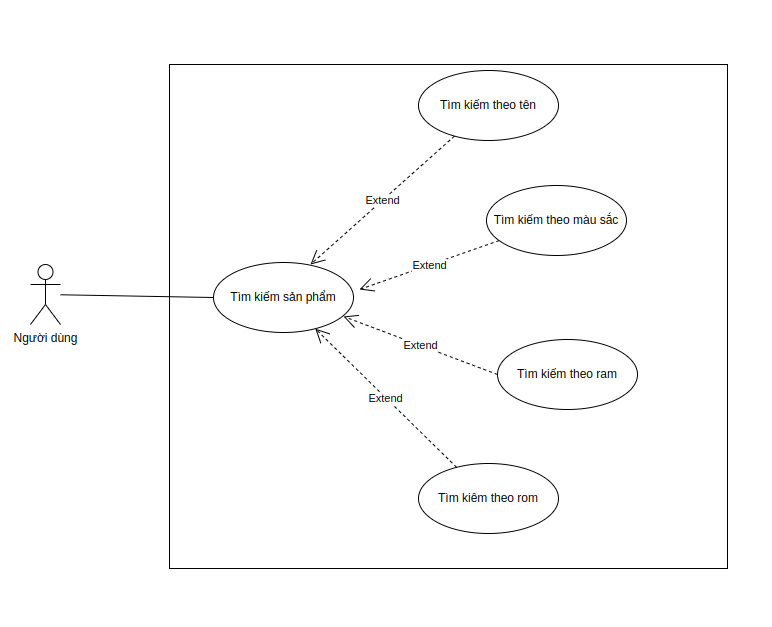
\includegraphics[scale=0.55]{Hinhve/search.png}
    \caption{Usecase phân rã tìm kiếm sản phẩm}
    \label{fig:my_label2}
\end{figure}

Chức năng tìm kiếm sản phẩm được phân rã thành các chức năng nhỏ hơn cho phép người dùng có thể linh hoạt tìm kiếm sản phẩm theo các tiêu chí khác nhau như tên sản phẩm, màu sắc của sản phẩm, dung lượng bộ nhớ trong (RAM), dung lượng bộ nhớ ngoài (ROM) 

\subsection{Quy trình nghiệp vụ}
\label{subsection:2.2.3}
Quy trình nghiệp vụ usecase tìm kiếm sản phẩm

% 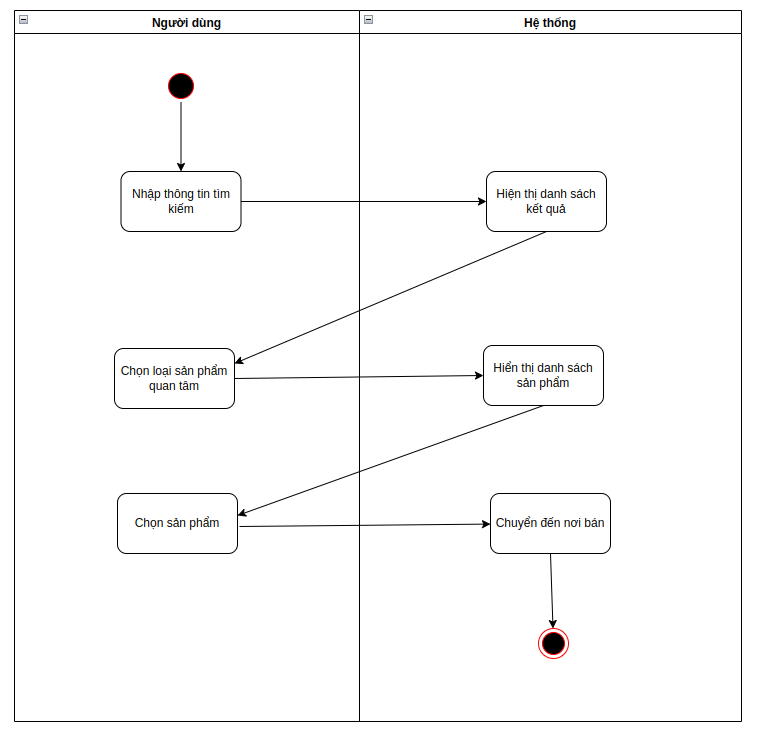
\includegraphics[scale=0.6]{Hinhve/quytrinhnghiepvu.png}
\begin{figure}[H]
    \centering
    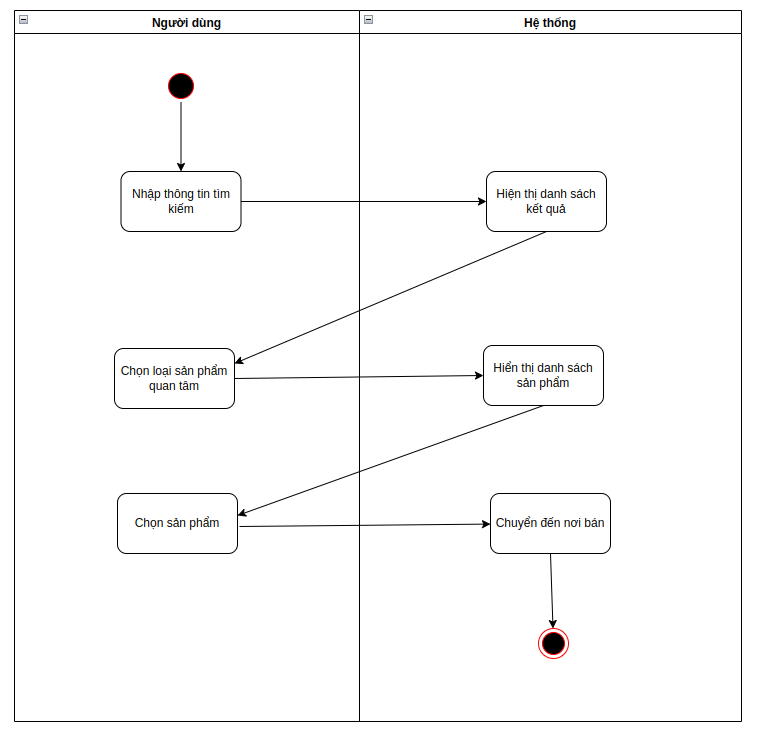
\includegraphics[scale=0.6]{Hinhve/quytrinhnghiepvu.png}
    \caption{Quy trình nghiệp vụ}
    \label{fig:my_label2}
\end{figure}

\section{Đặc tả chức năng}
\label{section:2.3}

\subsection{Đặc tả use case Tìm kiếm sản phẩm}



\begin{table}[H]
\centering{}
    \begin{tabular}{|l|}
    \hline
    Tên ca sử dụng: Tìm kiếm sản phẩm \\
    \hline
    Tác nhân chính: Người sử dụng phần mềm\\
    \hline
    Mục đích: Tìm kiếm sản phẩm mà người dùng quan tâm\\
    \hline
    Mô tả: Ca sử dụng mô tả cách người dùng tìm kiếm sản phẩm\\
    \hline
    Tiền điều kiện: Chuyển đến giao diện tìm kiếm sản phẩm\\
    \hline
    Hậu điều kiện: không có\\
    \hline
    Kích hoạt: Người dùng chọn chức năng Tìm kiếm sản phẩm\\
    \hline
    \makecell{Luồng sự kiện chính: \\
    
    1. Người dùng chọn chức năng tìm kiếm sản phẩm
    \\
    2. Người dùng nhập từ khóa để tìm kiếm sản phẩm theo tên, màu, ram, rom,..
    \\
    3. Người dùng bấm nút Tìm kiếm
    \\
    4. Hệ thống tìm kiếm và lấy về danh sách sản phẩm thỏa mãn điều kiện tìm kiếm.
    \\
    5. Hệ thống hiển thị danh sách sản phẩm tìm kiếm}
    \\
    \hline
    Luồng sự kiện ngoại lệ: 2.a Người dùng không nhập từ khóa tìm kiếm 
    \\
    \hline
    \end{tabular}
    \caption{Đặc tả usecase Tìm kiếm sản phẩm}
    \label{fig:my_label}
\end{table}

\hfill
\subsection{Đặc tả use case Xem thông tin sản phẩm}



\begin{table}[H]
\centering{}
    \begin{tabular}{|l|}
    \hline
    Tên ca sử dụng: Xem thông tin sản phẩm \\
    \hline
    Tác nhân chính: Người sử dụng phần mềm\\
    \hline
    Mục đích: Xem thông tin sản phẩm mà người dùng quan tâm\\
    \hline
    Mô tả: Ca sử dụng mô tả cách người dùng Xem thông tin sản phẩm\\
    \hline
    Tiền điều kiện: Chuyển đến giao diện Xem thông tin sản phẩm\\
    \hline
    Hậu điều kiện: không có\\
    \hline
    Kích hoạt: Người dùng chọn chức năng Xem thông tin sản phẩm\\
    \hline
    \makecell{Luồng sự kiện chính: \\
    
    1. Người dùng chọn chức năng Xem thông tin sản phẩm
    \\
    2. Người dùng chọn sản phẩm và xem thông tin sản phẩm
    \\
    3. Hệ thống tìm kiếm và lấy về danh sách thông tin kĩ thuật về sản phẩm
    \\
    4. Hệ thống hiển thị danh sách thông tin của sản phẩm}
    \\
    \hline
    Luồng sự kiện ngoại lệ: không có
    \\
    \hline
    \end{tabular}
    \caption{Đặc tả usecase xem thông tin sản phẩm}
    \label{fig:my_label}
\end{table}

\hfill
\subsection{Đặc tả use case xem biểu đồ}

\begin{table}[H]
\centering{}
    \begin{tabular}{|l|}
    \hline
    Tên ca sử dụng: Xem biểu đồ \\
    \hline
    Tác nhân chính: Người sử dụng phần mềm\\
    \hline
    Mục đích: Xem Xem biểu đồ  mà người dùng quan tâm\\
    \hline
    Mô tả: Ca sử dụng mô tả cách người dùng Xem biểu đồ \\
    \hline
    Tiền điều kiện: Chuyển đến giao diện Xem biểu đồ \\
    \hline
    Hậu điều kiện: không có\\
    \hline
    Kích hoạt: Người dùng chọn chức năng Xem biểu đồ \\
    \hline
    \makecell{Luồng sự kiện chính: \\
    
    1. Người dùng chọn chức năng Xem biểu đồ 
    \\
    2. Người dùng chọn biểu đồ và xem thông tin
    \\
    3. Hệ thống tạo biểu đồ
    \\
    4. Hệ thống hiển thị biểu đồ }
    \\
    \hline
    Luồng sự kiện ngoại lệ: không có
    \\
    \hline
    \end{tabular}
    \caption{Đặc tả usecase xem biểu đồ}
    \label{fig:my_label}
\end{table}


\section{Yêu cầu phi chức năng}
\label{section:2.4}
Hệ thống có giao diện đơn giản dễ sử dụng, ngôn ngữ Tiếng Viêt, thời gian phản hồi yêu cầu không quá 3s. Hệ thống cơ sở dữ liệu luôn có sẵn (không có thời gian chết) để phục vụ truy vấn mọi lúc.

%%%%%%%%%%%%%%%%%%%%%%%%%%%%%%%%%%%
Chương này đã phân tích khảo sát yêu cầu cũng như mô tả các chức năng cần có của hệ thống so sánh giá. Từ kết quả khảo sát em đã thực hiện cách tiếp cận xây dựng hệ thống data warehouse để đồng bộ và tích hợp dữ liệu. Để xây dựng một hệ thống hoàn chỉnh này, em có sử dụng một vài công nghệ thu thập, lưu trữ, xử lý sẽ được giới thiệu trong Chương 3

\end{document}